\documentclass[11pt]{article}

\usepackage{amsmath}
\usepackage{amssymb}
\usepackage[colorlinks=true, citecolor=blue, linkcolor=black]{hyperref}
\usepackage{listings}
\usepackage{xcolor}
\usepackage{graphicx}
\usepackage{caption}
\usepackage{subcaption}
\lstset { %
    language=C++,
    backgroundcolor=\color{black!5}, % set backgroundcolor
    basicstyle=\footnotesize,% basic font setting
    morekeywords={lu, solve, trimatl, trimatu},
    tabsize = 2,
}

\title{FYS3150 Project 1}
\date{Fall 2015}
\author{Ole Gunnar Johansen}

\begin{document}
	\maketitle
	
	\begin{abstract}
		In this project, I have investigated numerical methods of solving a set of linear equations. The specific example used is Poisson's equation known from electromagnetism. This report concerns two numerical methods for solving this problem - one involving the computer heavy LU-decomposition and one method and algorithm developed specifically for the purpose of this project, but is also applicable to a wide variety of physical problems. The latter uses a total of $O(10n)$ FLOPS wheras the other uses $O(n^3)$ FLOPS, resulting in computer overflow at a relatively early stage compared in comparison, and in turn, resulting in a much longer time spent computing.
	\end{abstract}
	
	\section{Introduction}
		In reality, the time available for computing is greatly limited by a number of factors. It is therefore of great interest to lower this as much as possible, while at the same time maintaining an acceptable degree of error. To investigate this, I have in this project solved a set of linear equations involving Poisson's equation known from electromagnetism. I first implemented functions from the open-sourced C++ library Armadillo to solve the equations using LU-decomposition and a form of gaussian elimination before I embarked on creating my own functions which exploits the tridiagonal nature of the matrix involved in the equations. 
		
		The two methods are discussed in detail in the Methods section, and in light of the errors and computing times listed in the Results section, I end the report by discussing the effectiveness of the two methods.
		
		All programs can be found at my github at \cite{github}, or, in case this is not yet set up, the dropbox folder at \cite{dropbox}.
	
	
	\section{Method}
		The Poisson-equation in three dimensions with spherical symmetry is a one-dimensional one in the variable $r$:
		\begin{align}
			\frac{1}{r^2}\frac{d}{dr}\left( r^2 \frac{d\Phi}{dr} \right) = -4\pi\rho(r)
		\end{align}
		Rewriting this using the substitution $\Phi(r) = \psi(r)/r$, we obtain 
		\begin{align}
			\frac{d^2\phi}{dr^2} = -4\pi r \rho(r).
		\end{align}
		Further simplification by letting $\phi \rightarrow u$, $r \rightarrow x$ and absorbing the constant $4\pi$ in a function $f$, we get the general one-dimensional Poisson-equation:
		\begin{align}
			-u''(x) = f(x)
		\end{align}
		
		I will now continue to discuss the one-dimensional Poisson-equation using Dirichlet boundary conditions with $x\in (0, 1)$ and $u(0)=u(1)=0$. We can approximate the second derivative of $u$ with
		\begin{align}
			-\frac{v_{i+1} + v_{i-1} - 2v_i}{h^2} = f_i \qquad \mathrm{for} \ i = 1,2,...,n \label{eq discete second derivative}
		\end{align}
		where $v_i$ is the discretized form of $u$ with grid points $x_i = ih$ and the step length $h=1/(n+1)$.
		
		By letting $b_i = h^2 f_i$ we can write out the terms of eq.~\eqref{eq discete second derivative}:

		\begin{align}
			\begin{matrix}	i=1 		&		&	2v_1		&	-	&	v_2		&		&			&					&		&				\\
									i=2		&		&	-v_1		&	+	&	2v_2		&	+	&	v_3	&					&		&				\\
									\vdots	&		&				&		&				&		&			&	\ddots 		&		&				\\
									i=n		&		&				&		&				&		&			&	-v_{n-1}	&	+	&	2v_n	
			\end{matrix} \quad
			\begin{matrix}
				= & \tilde{b_1} \\
				= & \tilde{b_2} \\
				\vdots & \\
				= & \tilde{b_n}
			\end{matrix}
		\end{align}
		
		or, equivalently as the linear equation
		\begin{align}
			\hat{A}\mathbf{v} = \mathbf{\tilde{b}}
		\end{align}
		where $\mathbf{v} = (v_1, v_2, ..., v_n)^T$, $\mathbf{\tilde{b}} = (\tilde{b_1}, \tilde{b_2}, ..., \tilde{b_n})^T$ and
		\begin{align}
			\hat{A} =
			\begin{pmatrix}
				2	&	-1		&	0		&	\dots		&	\dots		&	0 			\\
				-1	&	2		&	-1		&	0			&	\dots		&	\dots		\\
				0	&	-1		&	2		&	-1			&	0			&	\dots		\\
					&	\dots	&	\dots	&	\dots		&	\dots		&	\dots		\\
				0	&	\dots	&			&	-1			&	2			&	-1			\\
				0	&	\dots	&			&	0			&	-1			&	2
			\end{pmatrix} \label{eq tridiagonal}
		\end{align}
		
		\subsection{Method 1: LU-Decomposition}
			The easiest method to implement in a numerical solver for linear equations is one that already exists. The C++ library Armadillo includes such capabilities in its \texttt{lu(L,U,A)} and \texttt{solve(A, x, b)}-functions. These are, however, not specifically designed for a tridiagonal matrix as in eq. \eqref{eq tridiagonal} but work for any (square) matrix of, in theory, any size.
			
			To do an LU-decomposition of the matrix $\hat{A}$, one must find the lower triangular matrix $\hat{L}$ which contains ones along its main diagonal, and the upper triangular matrix $\hat{U}$ such that their product equal $\hat{A}$:
			\begin{align}
				\hat{A} = \hat{L}\hat{U}
			\end{align}
			There is an algorithm for doing this is not included in this text, however, it can be found in this course's lecture notes\cite{comphysLectureNotes}. The computational aspect of interest is the number of FLOPS and for LU-decomposition this number goes as $O(n^3)$.
			
			Recall the original problem:
			\begin{align*}
				\hat{A}\mathbf{v} = \mathbf{\tilde{b}}
			\end{align*}
			Using the LU-decomposition of $\hat{A}$ we can write this as
			\begin{align*}
				\hat{A}\mathbf{v} = \mathbf{\tilde{b}} \quad \rightarrow \quad \hat{L}\hat{U}\mathbf{v} = \mathbf{\tilde{b}} \quad \rightarrow \quad \begin{cases} \hat{U}\mathbf{v} = \mathbf{w} \\ \hat{L}\mathbf{w} = \mathbf{\tilde{b}} \end{cases}
			\end{align*}
			The next step is to perform a forward substitution on the lower-triangular matrix equation $\hat{L}\mathbf{w} = \mathbf{\tilde{b}}$ and finally a backward substitution of the system $\hat{U}\mathbf{v} = \mathbf{w}$. Below is a code snippet of how this is implemented. \texttt{L}, \texttt{U}, \texttt{A}, \texttt{w}, \texttt{b\_tilde} and \texttt{v} are armadillo matrices and vectors. By calling the \texttt{trimatl} and \texttt{trimatu} functions, the \texttt{solve} function knows whether the systems are upper or lower triangular and allows for faster computation.
			
			\begin{lstlisting}
	lu(L, U, A);
	solve(w, trimatl(L), b_tilde);
	solve(v, trimatu(U), w);
			\end{lstlisting}
			This last bit goes as $O(n^2)$ FLOPS, resulting in a total number of FLOPS for the LU-decomposition method of $\sim n^3$ for large $n$.
		
		
		\subsection{Method 2: Own method}
			Since the particular matrix in question is tridiagonal, a much more effective algorithm can be implemented: both storage-wise and FLOPS-wise. Let the main diagonal be a vector $\mathbf{b}$ of length $n$, and the two semi-major diagonals be vectors $\mathbf{a}$ and $\mathbf{c}$ both with length $n-1$. A $4\times 4$-system would then look like this:
			\begin{align}
				\begin{pmatrix}
					b_1	&	c_1	&	0		&	0		\\
					a_2	&	b_2	&	c_2	&	0		\\
					0		&	a_3	&	b_3	&	c_3	\\
					0		&	0		&	a_4	&	b_4	
				\end{pmatrix}
				\begin{pmatrix}
					v_1	\\	v_2	\\	v_3	\\	v_4
				\end{pmatrix}
				=
				\begin{pmatrix}
					\tilde{b}_1 \\ \tilde{b}_2	\\	\tilde{b}_3	\\	\tilde{b}_4
				\end{pmatrix}
			\end{align}			 
			or equivalently:
			\begin{align*}
				\begin{matrix}
					b_1v_1	&	+	&	c_1v_2		&		&					&		&\\
					a_2v_1	&	+	&	b_2v_2		&	+	&	c_2v_3		&		&\\
								&		&	a_3v_2		&	+	&	b_3v_3		&	+	&	c_3v_4  \\
								&		&					&		&	a_4v_3 	&	+	&	b_4v_4 
				\end{matrix} \
				\begin{matrix}
					= \tilde{b}_1 	&	[1]\\
					= \tilde{b}_2 	&	[2]\\
					= \tilde{b}_3 	&	[3]\\
					= \tilde{b}_4	&	[4]
				\end{matrix}
			\end{align*}
			We will now use a forward elimination process to eliminate the elements along the lower semi-diagonal in matrix $\hat{A}$. First take $b_1\cdot \mathrm{eq. \ [2]} - a_2 \cdot \mathrm{eq. \ [1]}$. Equation [2] then becomes 
			\begin{align*}
				& (b_1b_2 - a_2c_1)v_2 + b_1c_2v_3 = b_1\tilde{b}_2 - a_2\tilde{b}_1 \\
				\rightarrow \qquad & b_2'v_2 + c_2' v_3 = \tilde{b}_2'
			\end{align*}
			Now, we will take $b_2' \cdot \mathrm{eq. \ [3]} - a_3 \cdot \mathrm{eq. \ [2]_{mod}}$ where eq. [2]$_\mathrm{mod}$ is the modified version of eq. [2]. We will then obtain the modified version of eq. [3] of the form:
			\begin{align*}
				b_3'v_3 + c_3'v_4 = \tilde{b}_3'
			\end{align*}
			Continue the pattern and return to matrix form, we have a new matrix where all elements in $\mathbf{a}$ have been eliminated and the other diagonals consist of the vectors $\mathbf{b'}$ and $\mathbf{c}'$. The algorithm is as follows:\\
			\begin{center}
				\begin{tabular}{rlll}
					$i = 1$:					&	$b_1' = b_1$								&	$c_1' = c_1$				&	$\tilde{b}_1' = \tilde{b}_1$ \\
					$i = 2, 3, ..., n$:	&	$b_i' = b_{i-1}'b_i - a_ic_{i-1}'$		&	$c_i' = b_{i-1}'c_i$	&	$\tilde{b}_i' = b_{i-1}'\tilde{b}_i - a_i \tilde{b}_{i-1}'$
				\end{tabular}	
			\end{center}
			where the last iteration would yield the equation $b_n'v_n = \tilde{b}_n'$ which in turn can be used in the backward substitution process to obtain the other elements of the vector $\mathrm{v}$. The backward substitution algorithm is much simpler:
			\begin{center}
				\begin{tabular}{rl}
					$i = n$:								&	$v_n = \frac{\tilde{b}_n'}{b_n'}$ \\[9pt]
					$i = (n-1), (n-2), ..., 1$:		&	$v_i = \frac{\tilde{b}_i' - c_i'v_{i+1}}{b_i'}$
				\end{tabular}
			\end{center}
			This method has a FLOP counting as $\sim O(10n)$ - remarkably less than the LU-method discussed above.
			I end this methods discussion with the above algorithms implemented in the C++ programming language:
			\begin{lstlisting}
	void forward_substitution(double* &a, double* &b, 
							double* &c, double* &b_tilde, int n){
		for (int i = 1; i < n; i++){
			b[i] = b[i-1]*b[i] - a[i]*c[i-1];
			c[i] = b[i-1]*c[i];
			b_tilde[i] = b[i-1]*b_tilde[i] - a[i]*b_tilde[i-1];
		}
	} // End: function forward_substitution

	void backward_substitution(double* &b, double* &c, 
							double* &b_tilde, double* &v, int n){
		v[n-1] = b_tilde[n-1]/b[n-1];
		for (int i = n-2; i >= 0; i--){
			v[i] = (b_tilde[i] - c[i]*v[i+1])/b[i];
		} // End: function backward_substitution
	}
			\end{lstlisting}
			


	\section{Results}
		Table~\ref{table comp times} shows how the number of grid points $n$ relates to the time spent computing for the two methods described above. As expected, the method implementing LU-decomposition dramatically increases its time spent computing, compared to method 2 where the tridiagonality of the matrix was used. 
		
		A numerical solution will, due to loss of numerical precision and the very fact of the approximation made in eq.~\ref{eq discete second derivative}, never be an exact solution. For calculating this error, it is useful to use the log of the absolute error, or in other words:
		\begin{align*}
			\epsilon_i = \log_{10}\left( \left| \frac{v_i - u_i}{u_i} \right| \right) 
		\end{align*}
		Table~\ref{table errors} shows the maximum of this function for the cases $n=10, 100, 1000, 10000, 10^5$ for the two methods implemented.
		
		In some cases, an increase in time spent computing can be exchanged for precision, however, table~\ref{table errors} show that the two methods produce exactly the same errors with respect to the analytical solution. Figure~\ref{fig:animals} show the numerical results plotted together with the analytical solution, and so it it obvious that, if the purpose is solely visual, $n=100$ is far enough.
		
		
		\begin{table}[h]
			\begin{center}
			\caption{Using method 2, the computational time can be reduced drastically for large values of $n$ (number of grid points). The times shown in this table are the averages over 10 computations.}
			\label{table comp times}
			\begin{tabular}{|c|c|c|}
				\hline
				$n$			&	Method 1: LU-decomposition	&	Method 2: Own method		\\ \hline
				10				&	$4.59\cdot 10^{-5}$ s				&	$4.95 \cdot 10^{-5}$ s			\\
				100			&	$2.3 \cdot 10^{-4}$ s					&	$4.92 \cdot 10^{-5}$ s			\\
				1000			&	$0.016$ s									&	$1.5 \cdot 10^{-4}$ s				\\
				10000		&	$2.2$ s										&	$9.3 \cdot 10^{-4}$ s				\\
				$10^5$		&	OVERFLOW							&	$8.4 \cdot 10^{-3}$ s				\\ \hline
			\end{tabular}
			\end{center}
		\end{table}
		
		\begin{table}[h]
			\begin{center}
				\caption{Errors. The log of the absolute error decreases as $n$, the number of grid points, increases. There is no difference up to and including the 5th decimal place between the two methods on the error with of the numerical solution with respect to the analytical solution. No further decimals were checked.}
				\label{table errors}
				\begin{tabular}{|c|c|c|}
					\hline
					$n$		&	Method 1: LU-decomposition	&	Method 2: Own method		\\ \hline
					10			&	$-1.18$										&	$-1.18$									\\
					100		&	$-3.09$										&	$-3.09$									\\
					1000		&	$-5.08$										&	$-5.08$									\\
					10000	&	$-6.79$										&	$-6.79$									\\
					$10^5$	&	OVERFLOW							&	$-7.00$									\\ \hline
				\end{tabular}
			\end{center}
		\end{table}
		
		\begin{figure}
 		   \centering
		    \begin{subfigure}[b]{0.4\textwidth}
        		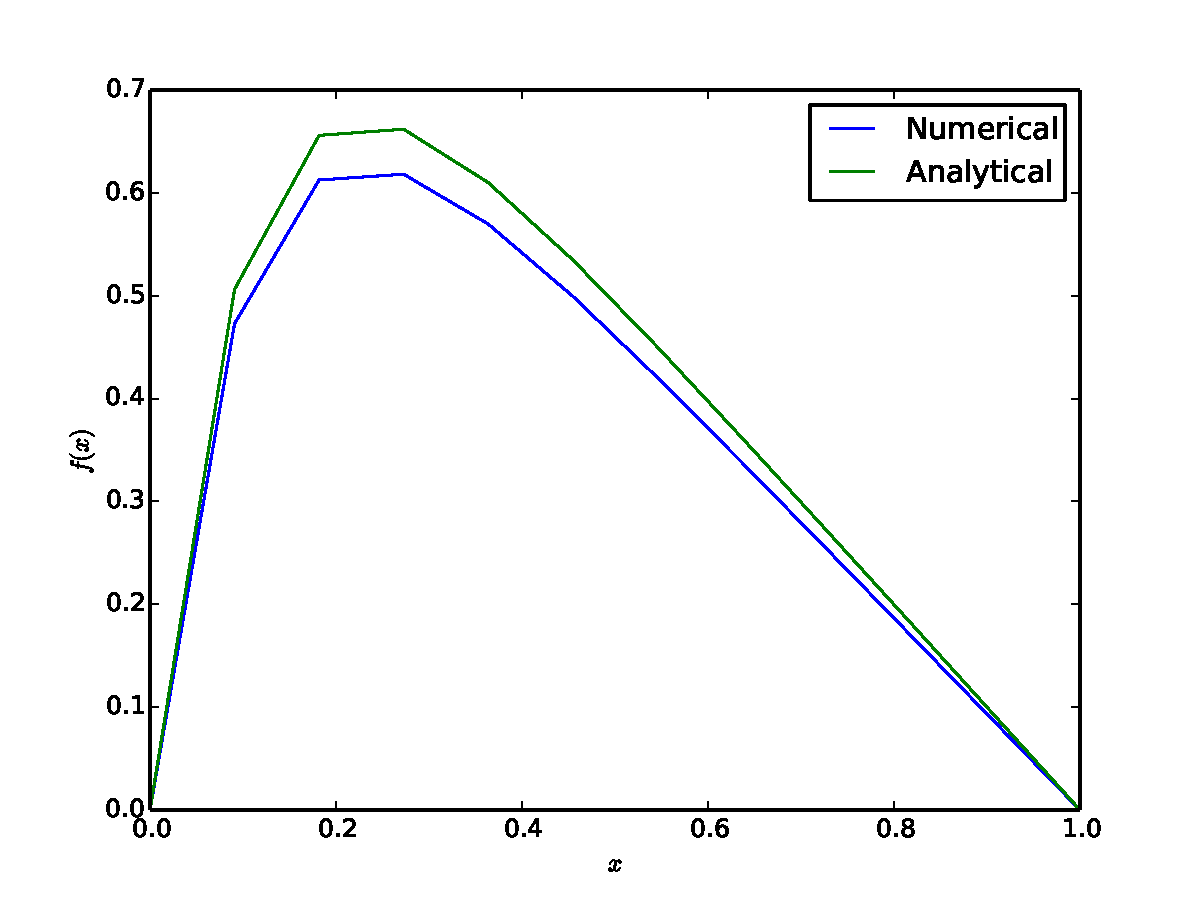
\includegraphics[scale=0.4, clip=true, trim= 50 0 0 0]{FYS3150_project_1_figure_n_10}
  		      \caption{$n = 10$}
 		       \label{fig:gull}
		    \end{subfigure}
		    \qquad \qquad \quad %add desired spacing between images, e. g. ~, \quad, \qquad, \hfill etc. 
		      %(or a blank line to force the subfigure onto a new line)
		    \begin{subfigure}[b]{0.4\textwidth}
		        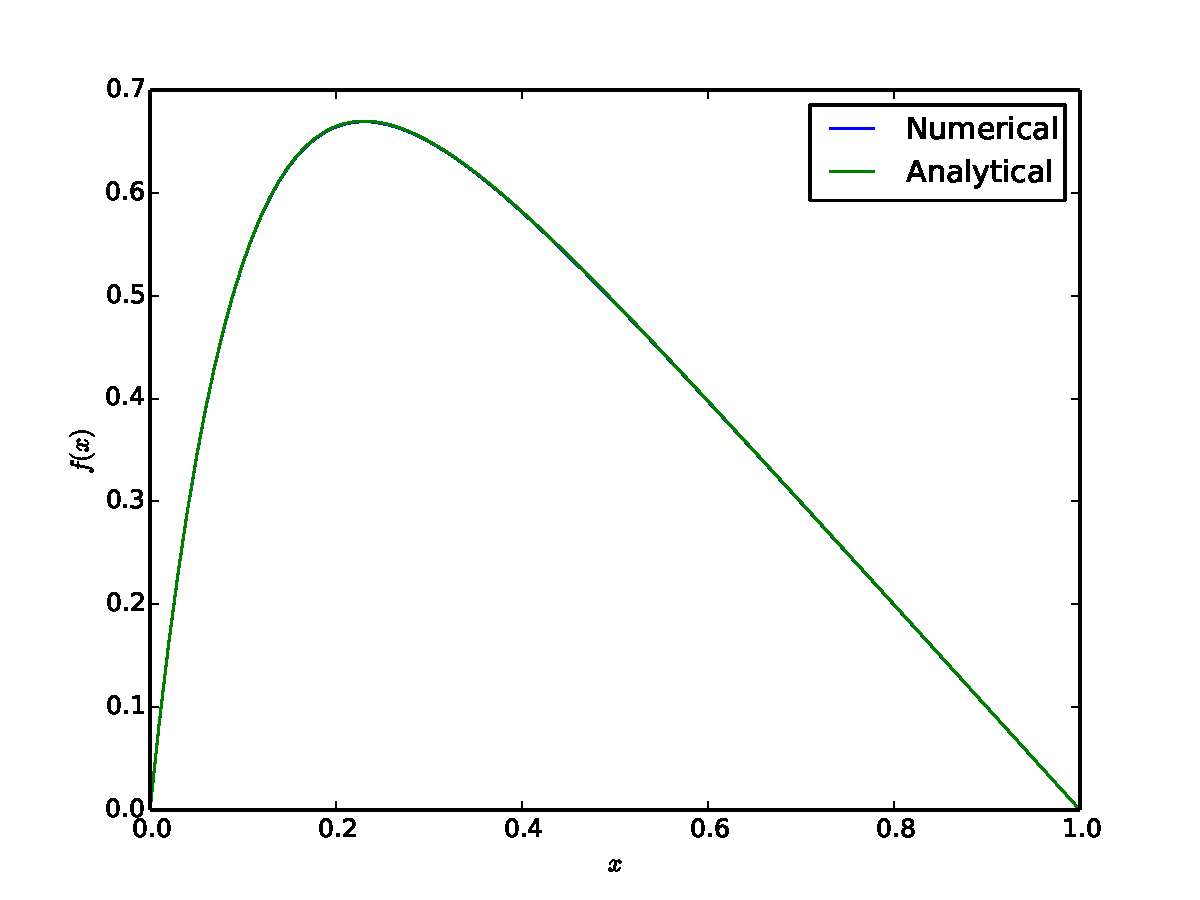
\includegraphics[scale=0.4, clip=true, trim= 50 0 0 0]{FYS3150_project_1_figure_n_100}
		        \caption{$n = 100$}
		        \label{fig:tiger}
		    \end{subfigure}
		    \caption{The analytical solution plotted vs. the numerical. It is obvoius that already at $n=100$, there is little or none visual difference between the two, indicating a good method and/or a relatively easy problem to do numerically.}\label{fig:animals}
		\end{figure}
		
	\section{Conclusion}
		As one might expect, the LU-decomposition method falls into a pit hole of overflow for large $n$. A discussed, this is due to the nature of LU-decomposition which requires $O(n^3)$ floating point operations. Trying to execute the program with $10^5$ grid points would then require $10^{15}$ FLOPS, in turn requiring a tremendous amount of memory in the computer. Also, we have shown that the problem can, without loss of precision, be solved in a manner requiring $O(n^2)$ less FLOPS resulting in a much higher precision possible and a lot less computer time needed. This method, or similar should therefore always be used then dealing with large tridiagonal matrix problems.
		
	\bibliographystyle{plain}
	\bibliography{references.bib}	
	
\end{document}